\documentclass[tikz,border=12pt]{standalone}
\usepackage[utf8]{inputenc}
\usepackage[T1]{fontenc}
\usepackage{amsmath,amssymb}
\usepackage{tikz}
\usepackage{pgfplots}
\pgfplotsset{compat=1.18}
\usepgfplotslibrary{groupplots}
\usetikzlibrary{arrows.meta,positioning,calc,backgrounds}

% V6 pastel-first palette
\definecolor{CoreNavy}{RGB}{72,92,120}
\definecolor{MutedBlue}{RGB}{104,132,164}
\definecolor{MutedRust}{RGB}{174,112,96}
\definecolor{MutedTeal}{RGB}{92,146,142}
\definecolor{PaleBlue}{RGB}{235,241,247}
\definecolor{PaleTeal}{RGB}{232,244,242}
\definecolor{PalePeach}{RGB}{248,238,231}
\definecolor{PaleRose}{RGB}{247,235,235}
\definecolor{SoftGray}{RGB}{244,245,246}
\definecolor{MidGray}{RGB}{153,160,168}
\definecolor{Ink}{RGB}{40,45,52}

\tikzset{
  module/.style={
    draw=CoreNavy,
    fill=SoftGray,
    line width=0.8pt,
    rounded corners=2mm,
    inner xsep=3.5mm,
    inner ysep=2.2mm,
    font=\sffamily\footnotesize,
    text=Ink,
    align=center
  }
}

\begin{document}
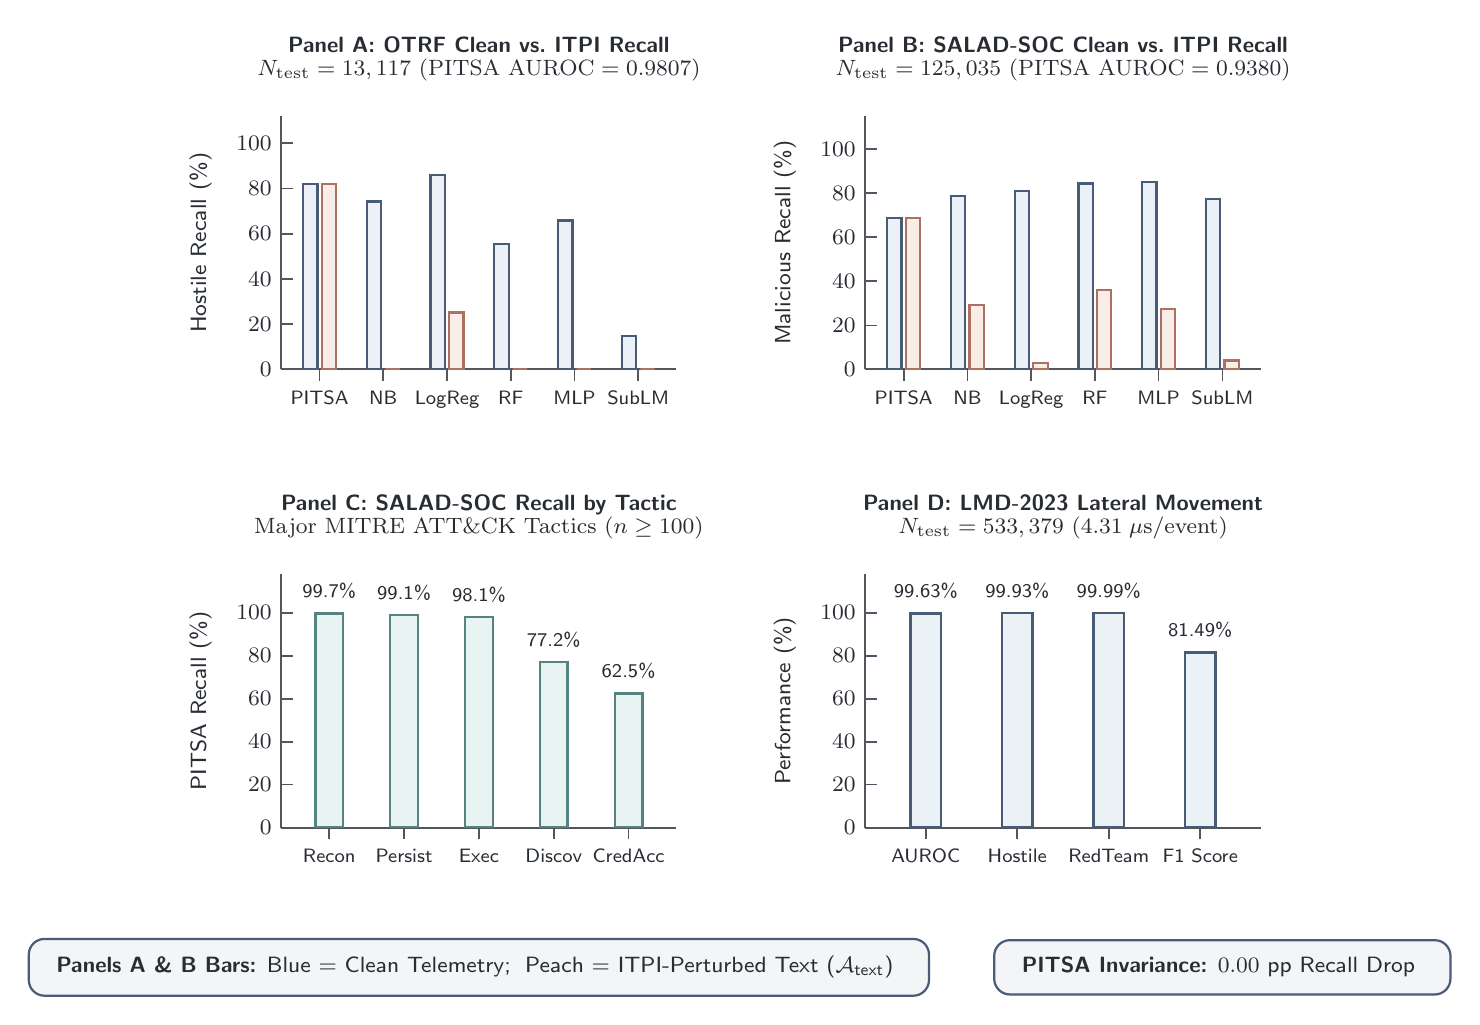
\begin{tikzpicture}[node distance=12mm and 14mm]

\begin{groupplot}[
  group style={
    group size=2 by 2,
    horizontal sep=24mm,
    vertical sep=26mm
  },
  width=66mm,
  height=48mm,
  grid=none,
  axis lines*=left,
  axis line style={draw=Ink!80, line width=0.7pt},
  tick style={draw=Ink!80, line width=0.6pt},
  tick label style={font=\sffamily\footnotesize, text=Ink},
  ylabel style={font=\sffamily\footnotesize, text=Ink, yshift=2pt},
  title style={font=\sffamily\footnotesize\bfseries, text=Ink, align=center, yshift=3pt}
]

% Panel A: OTRF Clean vs ITPI Recall (%)
\nextgroupplot[
  title={Panel A: OTRF Clean vs.\ ITPI Recall\\[-1pt]\normalfont\footnotesize $N_{\text{test}}=13,117$ ($\text{PITSA AUROC}=0.9807$)},
  ylabel={Hostile Recall (\%)},
  ybar=1.5pt,
  ymin=0, ymax=112,
  ytick={0,20,40,60,80,100},
  symbolic x coords={PITSA,NB,LR,RF,MLP,SubLM},
  xtick={PITSA,NB,LR,RF,MLP,SubLM},
  xticklabels={PITSA,NB,LogReg,RF,MLP,SubLM},
  xticklabel style={align=center, font=\sffamily\scriptsize, text=Ink},
  enlarge x limits=0.12
]
\addplot[
  draw=CoreNavy,
  line width=0.8pt,
  fill=PaleBlue,
  bar width=5.2pt
] coordinates {
  (PITSA,81.94)
  (NB,74.19)
  (LR,85.81)
  (RF,55.48)
  (MLP,65.81)
  (SubLM,14.84)
};
\addplot[
  draw=MutedRust,
  line width=0.8pt,
  fill=PalePeach,
  bar width=5.2pt
] coordinates {
  (PITSA,81.94)
  (NB,0.00)
  (LR,25.16)
  (RF,0.00)
  (MLP,0.00)
  (SubLM,0.00)
};

% Panel B: SALAD-SOC Clean vs ITPI Recall (%)
\nextgroupplot[
  title={Panel B: SALAD-SOC Clean vs.\ ITPI Recall\\[-1pt]\normalfont\footnotesize $N_{\text{test}}=125,035$ ($\text{PITSA AUROC}=0.9380$)},
  ylabel={Malicious Recall (\%)},
  ybar=1.5pt,
  ymin=0, ymax=115,
  ytick={0,20,40,60,80,100},
  symbolic x coords={PITSA,NB,LR,RF,MLP,SubLM},
  xtick={PITSA,NB,LR,RF,MLP,SubLM},
  xticklabels={PITSA,NB,LogReg,RF,MLP,SubLM},
  xticklabel style={align=center, font=\sffamily\scriptsize, text=Ink},
  enlarge x limits=0.12
]
\addplot[
  draw=CoreNavy,
  line width=0.8pt,
  fill=PaleBlue,
  bar width=5.2pt
] coordinates {
  (PITSA,68.68)
  (NB,78.65)
  (LR,80.87)
  (RF,84.37)
  (MLP,84.93)
  (SubLM,77.46)
};
\addplot[
  draw=MutedRust,
  line width=0.8pt,
  fill=PalePeach,
  bar width=5.2pt
] coordinates {
  (PITSA,68.68)
  (NB,29.39)
  (LR,2.92)
  (RF,36.05)
  (MLP,27.53)
  (SubLM,4.03)
};

% Panel C: SALAD-SOC PITSA Recall by MITRE ATT&CK Tactic
\nextgroupplot[
  title={Panel C: SALAD-SOC Recall by Tactic\\[-1pt]\normalfont\footnotesize Major MITRE ATT\&CK Tactics ($n \ge 100$)},
  ylabel={PITSA Recall (\%)},
  ybar,
  ymin=0, ymax=118,
  ytick={0,20,40,60,80,100},
  symbolic x coords={Rec,Per,Exe,Dis,Cre},
  xtick={Rec,Per,Exe,Dis,Cre},
  xticklabels={Recon,Persist,Exec,Discov,CredAcc},
  xticklabel style={align=center, font=\sffamily\scriptsize, text=Ink},
  enlarge x limits=0.16,
  point meta=explicit symbolic,
  nodes near coords,
  every node near coord/.append style={
    font=\sffamily\scriptsize,
    text=Ink,
    anchor=south,
    yshift=1.5pt
  }
]
\addplot[
  draw=MutedTeal!85!Ink,
  line width=0.85pt,
  fill=PaleTeal,
  bar width=10pt
] coordinates {
  (Rec,99.66) [99.7\%]
  (Per,99.08) [99.1\%]
  (Exe,98.14) [98.1\%]
  (Dis,77.20) [77.2\%]
  (Cre,62.50) [62.5\%]
};

% Panel D: LMD-2023 Held-Out Performance (N_test = 533,379)
\nextgroupplot[
  title={Panel D: LMD-2023 Lateral Movement\\[-1pt]\normalfont\footnotesize $N_{\text{test}}=533,379$ ($4.31\;\mu\text{s/event}$)},
  ylabel={Performance (\%)},
  ybar,
  ymin=0, ymax=118,
  ytick={0,20,40,60,80,100},
  symbolic x coords={AUC,Rec,RT,F1},
  xtick={AUC,Rec,RT,F1},
  xticklabels={AUROC,Hostile,RedTeam,F1 Score},
  xticklabel style={align=center, font=\sffamily\scriptsize, text=Ink},
  enlarge x limits=0.22,
  point meta=explicit symbolic,
  nodes near coords,
  every node near coord/.append style={
    font=\sffamily\scriptsize,
    text=Ink,
    anchor=south,
    yshift=1.5pt
  }
]
\addplot[
  draw=CoreNavy,
  line width=0.85pt,
  fill=PaleBlue!70!PaleTeal,
  bar width=11pt
] coordinates {
  (AUC,99.63) [99.63\%]
  (Rec,99.93) [99.93\%]
  (RT,99.99) [99.99\%]
  (F1,81.49) [81.49\%]
};

\end{groupplot}

% Summary banner placed below the groupplot
\node[module, below=14mm of group c1r2.south] (legend_banner) {
  \textbf{Panels A \& B Bars:} Blue = Clean Telemetry;\; Peach = ITPI-Perturbed Text ($\mathcal{A}_{\text{text}}$)
};

\node[module, right=8mm of legend_banner] (seed_note) {
  \textbf{PITSA Invariance:} $0.00\text{ pp}$ Recall Drop
};

\end{tikzpicture}
\end{document}
